\chapter{Modern Lute Fretting}

If we return to the initial subject at the outset of this paper, the standard in tuning
for the sixteenth and early seventeenth centuries was meantone temperament.  Many
performing ensembles today choose to use quarter-comma meantone temperament because it
was a very common temperament at the time for keyboard instruments, and as I explained
in chapter one, resulted in harmonious, pure thirds.  As we have seen in the previous
chapter, none of the major sources on lute fretting employ intervals that are
completely meantone in nature, quarter-comma or otherwise.  Certain frets are might be
meantone, but all of them are not uniformly tuned in one kind of temperament.  For any
would-be lute players wishing to participate in ensembles today that are employing
meantone temperaments, they are going to need practical solutions to make their
instruments function in a meantone setting.

Because of the arrangement of semitones on a lute, meantone temperaments must be
executed differently than on other instruments.  Players in the sixteenth century
recognized this problem and proposed various ways of dealing with the problem.  Some of
them ultimately decided that the lute was simply an equal semitone instrument, or
others observed that it was simply different and that music sounding bad on one
instrument seemed to sound much better on a lute.\textit{ML:1}[45]  However, we are
still faced with the reality that lutes performed with other instruments in large and
small ensembles, all of which very likely used quarter-comma meantone temperament and
other varieties of meantone temperament.  So it seems to reason that players then had
found ways to deal with the problem at least in some way.

The different historical fretting solutions set forth in the previous chapter fall
short of a comprehensive solution to meantone fretting; therefore, we are left to find
solutions to problem ourselves. In this chapter, I will address the
issue of meantone temperaments in ensembles, specifically quarter-comma
meantone temperament because it is the most common temperament associated with music
from this period and it is also one of more problematic temperaments to realize on the
lute. I will look at quarter-comma meantone in three different contexts: 1) a continuo
ensemble with theorbo; 2) a continuo ensemble with lute; and 3) ensembles with lute or
theorbo in tablature notation.

The solutions proposed here will build on ideas we have seen from historical sources,
but will also incorporante alternative solutions, some of which are modern and
contradict the approaches of the history treatises. They include the use of
\textit{tastini} or ``little frets'' made of wood or ivory that only span one string
and can be glued on the fret board.  These small frets make it possible to have a
different kind of semitone on one string, such as a chromatic semitone, while the rest
of the strings all have the diatonic semitone.  A alternative involves the use of frets
placed angles so they are not parallel to the nut or bridge.  This results in a fret
that could be a diatonic semitone on one end and a chromatic one on the other end.  The
arguments against such solutions found in historical sources support the notion that
the practice was commonly used; however, it was problematic enough that some authors
sought to rally against it. Nevertheless, we must consider these solutions if we are
able to find a musically acceptable solution to the quarter-comma dilemma.

Every solution to the problem of meantone temperament on the lute is a kind of
compromise.  Less drastic solutions included alternative fingerings for certain notes
and varying the finger pressure of the left hand to alter the pitch.  Adjustments such
as these could make pitches more agreeable in a tempered setting and enable the
instruments to function in given meantone context.  There are many different
combinations of solutions that can enable a lute to play in a quarter-comma meantone
temperament, but as we shall see, each combination has a different effect on the
instrument's capabilities.

\section{The Lute in Ensembles}

Musicians who played fretted instruments in ensembles with other instruments,
especially keyboard instruments, during the late 16th or early 17th-century would have
needed to utilize quarter-comma meantone temperament.  This was the standard
temperament for keyboard instruments and most, if not all, of bowed string and wind
instruments as well. For lutes, the problem is that none of the available historical
fretting instructions mention quarter-comma meantone at all.  The fretting schemes that
were presented in the previous chapter make use of tempered frets, some of which fall
near sixth-comma meantone, but none use full quarter-comma meantone fifths or thirds.
Either the historical evidence is lacking or there were cases when a lute was tuned to a
different temperament than the rest of the ensemble.

Most musicians today are uncomfortable with the idea of deliberately playing in a
different temperament than the rest of the instruments in an ensemble, so lute players
have found ways in which to make quarter-comma meantone successful on their
instruments. While it is possible to realize this temperament on a lute or theorbo, it
can create other problems such as limiting the instrument's compass or some of its
idiomatic qualities.  Common left-hand chord shapes may not be possible in a
quarter-comma meantone temperament.  However, if the instrument is used in basso
continuo, the choice of chord shape is at the player's discretion, so long as it agrees
with the harmony.  Since the player has more control over the number of voices in the
chord and its location on the fretboard, it is easier to overcome the limitations of a
meantone fretting system when playing in ensembles.  In solo situations, where the
exact location of each pitch is dictated by the tablature, a quarter-comma temperament
could produce undesirable results and necessitate a different temperament such as
sixth-comma.

Before we examine meantone fretting in tablature, we can see how quarter-comma meantone
may be realized on the lute.  If we recall, the main feature of meantone temperaments
are thirds that are much closer to pure than Pythagorean tuning or equal temperament.
The two side-effects of this are narrow fifths, or fifths that are flatter than pure,
and unequal semitones, namely the diatonic and chromatic semitone.  For the keyboard,
this means choosing between an F$\sharp$ and a G$\flat$, or a D$\sharp$ and an
E$\flat$.  In any meantone temperament, these are two different notes.  When tuning a
keyboard, the choice between a chromatic or a diatonic semitone can be independently
from any other note on the instrument. It is possible to have an F$\sharp$, A$\flat$
and C$\sharp$ all on the same octave.  On the lute, this is not possible because fret
placement dictates the semitone size for all notes along that fret. For example, the
choice of a chromatic semitone on one course to yield a C$\sharp$ might force another
course to have G$\sharp$ instead of A$\flat$.

In temperaments with unequal semitones, a lutenist can only choose between a chromatic
or a diatonic semitone when placing frets on his or her instrument.  For example, if we
were fretting our instrument in quarter-comma meantone, the first fret would either be
a chromatic semitone or a diatonic one.  The choice of semitone is up to the player,
but the main consideration the player should make is whether or not any pitches on that
fret must either be chromatic or diatonic.  For a lute in standard G tuning, the second
course is tunned to D; therefore, the first fret of the D course could either be
E$\flat$ or D$\sharp$, the second fret of the course E and the third is F.  The
distance between E and F is a diatonic semitone which makes the distance between the
second and third fret a diatonic semitone.  Because of this one requirement in tuning
between two notes on a single course, the distance of a diatonic semitone between these
two frets will apply to all other courses as well.  Given these requirements, Dowland's
chromatic sixth-comma fret in table~\ref{table:comparison} seems impossible, because
this would create something flatter than F.  Gerle's diatonic fret, on the other hand,
makes more sense in this context.

The other consideration players can make when choosing semitone size is that some
chromatic notes are more common than others.  For example, it is more common to find an
F$\sharp$ in 17th-century music than it is a G$\flat$.  Returning to our previous example
of the D course, the fourth fret makes better sense as a chromatic semitone, giving us an
F$\sharp$, instead of a diatonic one which would have produced a G$\flat$.  If we use this
same logic and move back to the first fret of that course, we could choose an E$\flat$
over a D$\sharp$ by using the reasoning that we are probably more likely to encounter an
E$\flat$ than a D$\sharp$, although this is not always the case.

For the sake of argument, let us say that we have settled on the semitone choices we have
discussed above: diatonic first and third frets, followed by a chromatic forth fret.  The
result of these semitone sizes are summarized in figure~\ref{fig:quarter-diatonic}, and as
we can see, this has an interesting impact on the rest of the pitches on the other courses
of the same frets.
\begin{figure}[ht]
\centering
\setlength{\unitlength}{0.5mm}
\begin{picture}(60,191.6)
% Draw fingerboard edges
\color{black}
\linethickness{0.075mm}
\put(0,0){\line(0,1){186.6}}
\put(60,0){\line(0,1){186.6}}

% Draw strings
% 6th course
\color{strings}
\linethickness{0.5mm}
\put(5,0){\line(0,1){186.6}}
\linethickness{0.25mm}
\put(7,0){\line(0,1){186.6}}
% 5th course
\put(15,0){\line(0,1){186.6}}
\put(17,0){\line(0,1){186.6}}
% 4th course
\put(25,0){\line(0,1){186.6}}
\put(27,0){\line(0,1){186.6}}
% 3rd course
\put(35,0){\line(0,1){186.6}}
\put(37,0){\line(0,1){186.6}}
% 2nd course
\put(45,0){\line(0,1){186.6}}
\put(47,0){\line(0,1){186.6}}
% 1st course
\put(56,0){\line(0,1){186.6}}
% Insert string pitch names for lute in G
% 6th
\color{black}
\put(2,191.6){\small{G}}
% 5th
\put(14,191.6){\small{c}}
% 4th
\put(24,191.6){\small{f}}
% 3rd
\put(34,191.6){\small{a}}
% 2nd
\put(43,191.6){\small{d'}}
% 1st
\put(53,191.6){\small{g'}}
\color{black}
\linethickness{1mm}
\put(0,136.2){\line(1,0){60}}
\color{black}
\put(60,135.2){\small{\textemdash  1st (diatonic)}}
\color{black}
\linethickness{1mm}
\put(0,107.6){\line(1,0){60}}
\color{black}
\put(60,106.6){\small{\textemdash  2nd (chromatic)}}
\color{black}
\linethickness{1mm}
\put(0,41.3){\line(1,0){60}}
\color{black}
\put(60,40.3){\small{\textemdash  4th (chromatic)}}
\color{black}
\linethickness{1mm}
\put(0,5){\line(1,0){60}}
\color{black}
\put(60,4){\small{\textemdash  5th (diatonic)}}
\color{black}
\linethickness{1mm}
\put(0,66.9){\line(1,0){60}}
\color{black}
\put(60,65.9){\small{\textemdash  3rd (diatonic)}}
\color{black}
\linethickness{1mm}
\put(0,181.6){\line(1,0){60}}
\color{black}
\put(60,180.6){\small{\textemdash  Nut}}
\color{black}
\put(2,158.9){\small{A$\flat$}}
\put(12,158.9){\small{d$\flat$}}
\put(22,158.9){\small{g$\flat$}}
\put(32,158.9){\small{b$\flat$}}
\put(42,158.9){\small{e$\flat$'}}
\put(52,158.9){\small{a$\flat$'}}
\color{black}
\put(2,23.1){\small{c}}
\put(12,23.1){\small{f}}
\put(22,23.1){\small{b$\flat$}}
\put(32,23.1){\small{d'}}
\put(42,23.1){\small{g'}}
\put(52,23.1){\small{c''}}
\color{black}
\put(2,87.2){\small{B$\flat$}}
\put(12,87.2){\small{e$\flat$}}
\put(22,87.2){\small{a$\flat$}}
\put(32,87.2){\small{c'}}
\put(42,87.2){\small{f'}}
\put(52,87.2){\small{b$\flat$'}}
\color{black}
\put(2,54.1){\small{B}}
\put(12,54.1){\small{e}}
\put(22,54.1){\small{a}}
\put(32,54.1){\small{c$\sharp$'}}
\put(42,54.1){\small{f$\sharp$'}}
\put(52,54.1){\small{b'}}
\color{black}
\put(2,121.9){\small{A}}
\put(12,121.9){\small{d}}
\put(22,121.9){\small{g}}
\put(32,121.9){\small{b}}
\put(42,121.9){\small{e'}}
\put(52,121.9){\small{a'}}
\end{picture}
\caption{Standard quarter-comma fretting}
\label{fig:quarter-diatonic}
\end{figure}

Since we have chosen E$\flat$ over D$\sharp$ for the first fret, this results in a
B$\flat$ for the third course, which is a good choice; however, the fourth and fifth
courses are G$\flat$ and D$\flat$, instead of the more likely F$\sharp$ and C$\sharp$.
This also creates a problem because the G$\flat$ found on the first fret of the fourth
course will not match the F$\sharp$ on the fourth fret of the second course. Similarly,
the D$\flat$ on the fifth course will not match the C$\sharp$ on the third.

The alternative solution is to have a chromatic semitone for the first fret instead of a
diatonic one, seen in figure ~\ref{fig:quarter-chromatic}, but this only makes things
worse.
\begin{figure}[ht]
\centering
\setlength{\unitlength}{0.5mm}
\begin{picture}(60,191.6)
% Draw fingerboard edges
\color{black}
\linethickness{0.075mm}
\put(0,0){\line(0,1){186.6}}
\put(60,0){\line(0,1){186.6}}

% Draw strings
% 6th course
\color{strings}
\linethickness{0.5mm}
\put(5,0){\line(0,1){186.6}}
\linethickness{0.25mm}
\put(7,0){\line(0,1){186.6}}
% 5th course
\put(15,0){\line(0,1){186.6}}
\put(17,0){\line(0,1){186.6}}
% 4th course
\put(25,0){\line(0,1){186.6}}
\put(27,0){\line(0,1){186.6}}
% 3rd course
\put(35,0){\line(0,1){186.6}}
\put(37,0){\line(0,1){186.6}}
% 2nd course
\put(45,0){\line(0,1){186.6}}
\put(47,0){\line(0,1){186.6}}
% 1st course
\put(56,0){\line(0,1){186.6}}
% Insert string pitch names for lute in G
% 6th
\color{black}
\put(2,191.6){\small{G}}
% 5th
\put(14,191.6){\small{c}}
% 4th
\put(24,191.6){\small{f}}
% 3rd
\put(34,191.6){\small{a}}
% 2nd
\put(43,191.6){\small{d'}}
% 1st
\put(53,191.6){\small{g'}}
\color{black}
\linethickness{1mm}
\put(0,107.6){\line(1,0){60}}
\color{black}
\put(60,106.6){\small{\textemdash  2nd (chromatic)}}
\color{black}
\linethickness{1mm}
\put(0,41.3){\line(1,0){60}}
\color{black}
\put(60,40.3){\small{\textemdash  4th (chromatic)}}
\color{black}
\linethickness{1mm}
\put(0,5){\line(1,0){60}}
\color{black}
\put(60,4){\small{\textemdash  5th (diatonic)}}
\color{black}
\linethickness{1mm}
\put(0,151){\line(1,0){60}}
\color{black}
\put(60,150){\small{\textemdash  1st (chromatic)}}
\color{black}
\linethickness{1mm}
\put(0,66.9){\line(1,0){60}}
\color{black}
\put(60,65.9){\small{\textemdash  3rd (diatonic)}}
\color{black}
\linethickness{1mm}
\put(0,181.6){\line(1,0){60}}
\color{black}
\put(60,180.6){\small{\textemdash  Nut}}
\color{black}
\put(2,23.1){\small{c}}
\put(12,23.1){\small{f}}
\put(22,23.1){\small{b$\flat$}}
\put(32,23.1){\small{d'}}
\put(42,23.1){\small{g'}}
\put(52,23.1){\small{c''}}
\color{black}
\put(2,129.3){\small{A}}
\put(12,129.3){\small{d}}
\put(22,129.3){\small{g}}
\put(32,129.3){\small{b}}
\put(42,129.3){\small{e'}}
\put(52,129.3){\small{a'}}
\color{black}
\put(2,87.2){\small{B$\flat$}}
\put(12,87.2){\small{e$\flat$}}
\put(22,87.2){\small{a$\flat$}}
\put(32,87.2){\small{c'}}
\put(42,87.2){\small{f'}}
\put(52,87.2){\small{b$\flat$'}}
\color{black}
\put(2,166.3){\small{G$\sharp$}}
\put(12,166.3){\small{c$\sharp$}}
\put(22,166.3){\small{f$\sharp$}}
\put(32,166.3){\small{a$\sharp$}}
\put(42,166.3){\small{d$\sharp$'}}
\put(52,166.3){\small{g$\sharp$'}}
\color{black}
\put(2,54.1){\small{B}}
\put(12,54.1){\small{e}}
\put(22,54.1){\small{a}}
\put(32,54.1){\small{c$\sharp$'}}
\put(42,54.1){\small{f$\sharp$'}}
\put(52,54.1){\small{b'}}
\end{picture}
\caption{Alternate Quarter-comma Fretting for the Lute}
\label{fig:quarter-chromatic}
\end{figure}

It allows for an F$\sharp$, C$\sharp$ and G$\sharp$ on the lower courses, matching the
C$\sharp$ and F$\sharp$ of the fourth fret, but the D$\sharp$ and A$\sharp$ on the
upper courses proves to be a problem. A$\sharp$ is an especially unlikely chromatic
note and it does not match the B$\flat$ found on the third fret of the sixth course.

There are two main reasons why the alternative solution of a chromatic first fret is
undesirable. First, it seems that most of the historical sources agree that the first
fret was some kind of diatonic semitone.  Referring back to
table~\ref{table:comparison}, Dowland, Gerle, Ganassi and Bermudo all agreed that the
first fret was diatonic in nature. Although theirs was closer to sixth-comma than
quarter-comma, it indicates a preference for the diatonic semitone, or notes that have
the $\flat$ accidental as opposed to a $\sharp$ accidental.

The second reason that a chromatic first fret is unlikely is because it would create
false unisons between the B$\flat$ and the A$\sharp$ , as well as the E$\flat$ on the
fifth and the D$\sharp$ on the second. These unisons are quite common in lute
tablature, and comprise some of the most common chord shapes used in continuo playing.
A chromatic first fret would render those chords unplayable without additional
adjustments, making it unlikely that a chromatic semitone would be used in either a
solo or ensemble context.

\section{The Theorbo}

As lutes were used more and more in ensembles towards the end of the sixteenth century, a
new type of lute was invented specifically intended to play in ensembles.  The theorbo, as
it was called, was a much larger instrument and had additional bass strings that extended
beyond the length of the neck.  Although all kinds of lutes, including the theorbo, were
generally fretted the same way, the tuning of the theorbo presented other alternative
fretting solutions that were not available on the the lute.  The theorbo's nominal pitch
was almost always A, instead of the G as with other lutes of the time.  Technically, any
lute or theorbo can be tunned to any key, and it was not uncommon to find lutes pitched to
F, G, A and even D.  This applied to lutes in a consort where each existed in a variety of
sizes.  The pitch could also result from the instrument's mensur length.  The top string
would be tuned as high as possible without breaking and where that point was determined
the overall pitch of the instrument.

When taken in an ensemble context, the pitch of a lute or theorbo had to be
standardized so that it could play with other instruments.  In English consort music as
well as most all lute song publications in England, the standard lute pitched was G.
In Italy, however, the theorbo was usually pitched to A.  No matter the pitch of a
lute, courses were tuned so that the preceding course was always lower than the one
following it. (see figure~\ref{g-lute})  This was not the case for the theorbo and it
had first and second courses that were an octave lower. (see figure~\ref{a-theorbo})

\begin{figure}[h]
\centering
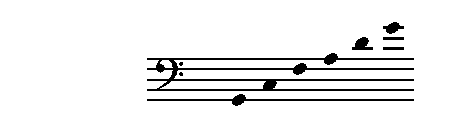
\includegraphics{examples/lute-tuning.pdf}
\caption{Standard lute tuning in G}
\label{g-lute}
\end{figure}
\begin{figure}[h]
\centering
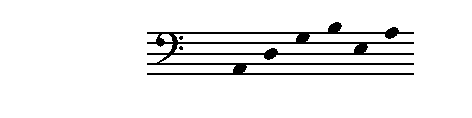
\includegraphics{examples/theorbo-tuning.pdf}
\caption{Theorbo tuned in A with re-entrant first and second courses}
\label{a-theorbo}
\end{figure}

Theorbos were designed for accompaniment and needed to provide more volume than other
lutes of the day; therefore, the body size was much larger and the strings were longer.
Because of the increased mensur length, it was not possible to preserve the low to high
arrangement of courses as they were on the lute. Players found that as they tried to tune
the upper strings to their normal lute pitches, the strings would break and it was not
possible to fashion a gut string thin enough to hold the pitch at that length.  To solve
the problem, they tuned the strings to the same pitch but at an octave lower and thus
preserving the same interval relationships between strings as they were on the lute  This
made chord shapes identical between instruments and only altered the voicings of the
chords. Since the theorbo was primarily a continuo instrument, the change in voicing did
not present a problem. In fact, it became more of an advantage.  The re-entrant tuning
kept the overall tessitura of the instrument lower and away from the accompanied singer or
instrumentalist.

All theorbos had eight additional bass strings that descended diatonically in pitch from
the A on the sixth course.  Therefore, the seventh, eighth and ninth courses would be G, F
and E, continuing on to an octave G on the fourteenth course.  The disposition of these
lower courses varied somewhat from instrument to instrument.  Praetorius discussed two
kinds of theorbos, one which he called a Roman style theorbo that had six courses on the
fretboard and all eight of the lower courses on the extended neck of the
instrument.\autocite[59]{MP:1} The other type, which he called the Paduan-style
theorbo, had eight courses on the fretboard and the rest of the bass courses were on the
extended neck.

Because of the variation Praetorius describes, players today will often have the seventh
as well as the eighth course on their fretboards before the additional strings on the
extended neck. See figure ~\ref{fig:theorbo-extended} below.
\begin{figure}[ht]
\centering
\setlength{\unitlength}{0.5mm}
\begin{picture}(80,191.6)
% Draw fingerboard edges
\color{black}
\linethickness{0.075mm}
\put(0,0){\line(0,1){186.6}}
\put(80,0){\line(0,1){186.6}}

% Draw strings
\color{strings}
\linethickness{0.5mm}
\put(5,0){\line(0,1){186.6}}
\put(15,0){\line(0,1){186.6}}
\put(25,0){\line(0,1){186.6}}
\put(35,0){\line(0,1){186.6}}
\put(45,0){\line(0,1){186.6}}
\put(55,0){\line(0,1){186.6}}
\put(65,0){\line(0,1){186.6}}
\put(75,0){\line(0,1){186.6}}

% Insert string pitch names for lute in A (theorbo)

\color{black}
\put(2,191.6){\small{F}}

\put(14,191.6){\small{G}}

\put(24,191.6){\small{A}}

\put(34,191.6){\small{d}}

\put(43,191.6){\small{g}}

\put(53,191.6){\small{b}}
\put(63,191.6){\small{e'}}
\put(73,191.6){\small{a'}}


\color{black}
\linethickness{1mm}
\put(0,136.2){\line(1,0){80}}
\color{black}
\put(80,135.2){\small{\textemdash  1st (diatonic)}}
\color{black}
\linethickness{1mm}
\put(0,107.6){\line(1,0){80}}
\color{black}
\put(80,106.6){\small{\textemdash  2nd (chromatic)}}
\color{black}
\linethickness{1mm}
\put(0,41.3){\line(1,0){80}}
\color{black}
\put(80,40.3){\small{\textemdash  4th (chromatic)}}
\color{black}
\linethickness{1mm}
\put(0,5){\line(1,0){80}}
\color{black}
\put(80,4){\small{\textemdash  5th (diatonic)}}
\color{black}
\linethickness{1mm}
\put(0,66.9){\line(1,0){80}}
\color{black}
\put(80,65.9){\small{\textemdash  3rd (diatonic)}}
\color{black}
\linethickness{1mm}
\put(0,181.6){\line(1,0){80}}
\color{black}
\put(80,180.6){\small{\textemdash  Nut}}
\color{black}
\put(2,158.9){\small{G$\flat$}}
\put(12,158.9){\small{A$\flat$}}
\put(22,158.9){\small{B$\flat$}}
\put(32,158.9){\small{e$\flat$}}
\put(42,158.9){\small{a$\flat$}}
\put(52,158.9){\small{c'}}
\put(62,158.9){\small{f'}}
\put(72,158.9){\small{b$\flat$'}}
\color{black}
\put(22,23.1){\small{d}}
\put(32,23.1){\small{g}}
\put(42,23.1){\small{c'}}
\put(52,23.1){\small{e'}}
\put(62,23.1){\small{a'}}
\put(72,23.1){\small{d''}}
\color{black}
\put(22,87.2){\small{c}}
\put(32,87.2){\small{f}}
\put(42,87.2){\small{b$\flat$}}
\put(52,87.2){\small{d'}}
\put(62,87.2){\small{g'}}
\put(72,87.2){\small{c''}}
\color{black}
\put(22,54.1){\small{c$\sharp$}}
\put(32,54.1){\small{f$\sharp$}}
\put(42,54.1){\small{b}}
\put(52,54.1){\small{d$\sharp$'}}
\put(62,54.1){\small{g$\sharp$'}}
\put(72,54.1){\small{c$\sharp$''}}
\color{black}
\put(22,121.9){\small{B}}
\put(32,121.9){\small{e}}
\put(42,121.9){\small{a}}
\put(52,121.9){\small{c$\sharp$'}}
\put(62,121.9){\small{f$\sharp$'}}
\put(72,121.9){\small{b}'}
\end{picture}
\caption{Theorbo with extend courses}
\label{fig:theorbo-extended}
\end{figure}

The advantage to having these additional courses on the neck is that a
player is able to fret additional chromatic notes with the left hand.  On the longer
strings that are attached to the extension, this is not possible and any chromatic changes
in the pitches of those stings must be done using the tuning pegs prior to playing.

While it might have been possible to tune a lute's first course to a chromatic semitone,
this was impossible on the theorbo. For example, the first fret had to be diatonic because
of the open E$\natural$ and B$\natural$ on the second and third courses so that the
pitches on those courses of the first fret would be F$\natural$ and C$\natural$.  If a
chromatic semitone was used, an E$\sharp$ and B$\sharp$ would result, making this type of
semitone unusable. Similarly, the presence of a B$\flat$ at the third fret of the fourth
course dictates that the next fret must be chromatic to create a B$\natural$ at the fourth
fret of the same course. Even the sixth fret is determined to be diatonic because of the
E$\natural$ to F$\natural$ that occurs on the third course.

Essentially, the frets of a theorbo tuned to meantone temperament were ``fixed'' in
their positions because the location of the diatonic semitones between B and C, and E
and F determined which fret was either chromatic or diatonic.  If we also take into
consideration the same issue of octaves that affect the position of frets on the lute
in G, it makes the most sense for a theorbo to have its frets arranged the same way as
a lute and alternate between diatonic and chromatic semitones, beginning with a
diatonic semitone at the first fret.  Since this limits the type of semitones that are
available, we have to find alternative methods of playing semitones if we are to be
successful in a quarter-comma meantone temperament.

\subsection{Solutions utilizing re-entrant tuning}

Because of the theorbo's unique re-entrant tuning, it has the potential advantage of using
both the chromatic and the diatonic semitones.  Notes that were normally an octave
apart on the lute were unisons on the theorbo.  This offered a possible solution to some
of the problems of semitone size because a particular pitch could be a diatonic semitone
at one fret, a chromatic one at a different fret and still be in the same octave. Referring
to figure~\ref{fig:theorbo-extended}, the A$\flat$ on the first fret of the fourth course
and the G$\sharp$ found on the fourth fret of the second course are in the same octave,
whereas on a lute in standard G tuning they are an octave apart. Similarly, the E$\flat$
on the fifth course of the first fret also has its chromatic counterpart D$\sharp$ on the
third course of the fourth fret.  All the player has to do is choose the appropriate
fingering for the left hand.

For chords that require chromatic semitones, such as a G$\sharp$ or a D$\sharp$, the
player can use pitches found on the fourth fret.  Some of the more common left-hand chord
patterns that use this fret include the E major triad and different kinds of chords with a
sixth above the bass.
\begin{figure}[h]
\centering
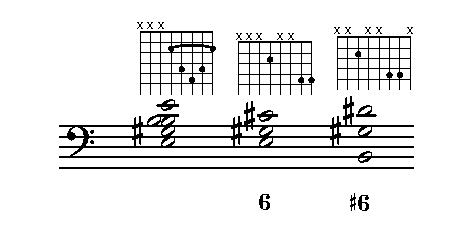
\includegraphics{examples/g-sharp.pdf}
\caption{Chords using chromatic semitones on the fourth fret}
\label{fourth-fret-chords}
\end{figure}
For other chords that require diatonic semitones, such as the A$\flat$ or E$\flat$, the
player may use pitches on the first fret.  This includes A$\flat$ major, F minor and C
minor.
\begin{figure}[h]
\centering
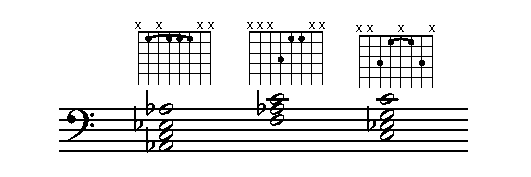
\includegraphics{examples/a-flat.pdf}
\caption{Chords using diatonic semitones on the first fret}
\label{first-fret-chords}
\end{figure}
Although instances of an A$\flat$ major triad are rare, all the needed pitches are on the
first fret and the F minor and C minor triads are both possible using a limited number of voices.

While re-entrant tuning makes it possible to play chords with different kinds of
semitones, the left-hand chord fingerings that result are not idiomatic to the instrument.
More ideal chords for the theorbo are easier to execute, use as many strings as possible,
and favor open strings whenever possible.  The fingerings for F minor and C minor listed
in figure~\ref{first-fret-chords} are not commonly found in existing theorbo tablatures of the time, nor are
they used very often among modern players. The more common fingerings for these chords
use the fourth fret.  Additionally, the E major chord in figure~\ref{fourth-fret-chords}
uses the chromatic semitone on the fourth fret, but ignores the open E and B on the third
and second courses. More common chord fingerings below in figure~\ref{common-chords} indicate that a player
would more likely use a fully-voiced F minor or C minor chord with a barre at the third
fret than those listed previously.  An E major chord that makes use of the open B and
E strings would sound much more resonant and would be easier to play for the left-hand.
\begin{figure}[h]
\centering
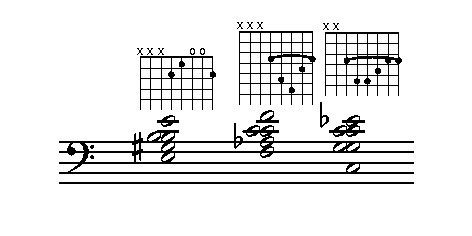
\includegraphics{examples/common-chords.pdf}
\caption{Common theorbo chord shapes}
\label{common-chords}
\end{figure}
The obvious problem with these more idiomatic chord shapes is that if they are used on
a theorbo in meantone temperament, their semitones are opposite of what they should be.
The E major chord shown above would have a diatonic A$\flat$ instead of the chromatic
G$\sharp$ and the thirds of the F minor and C minor chords would be chromatic in nature
instead of diatonic.

\subsection{Tastini}

The advantages that re-entrant tuning might offer has the side-effect of rendering our
more idiomatic chord shapes unusable in a meantone temperament.  If we want to be able to
use these shapes, yet still be able to play in meantone temperament, we need the ability
to locally apply different semitones within a fret instead of being forced to have all the
pitches at one fret of a certain size. In other words, we need to mix both chromatic and
diatonic semitone sizes within the same fret.  For example, consider the pitches of the
extended bass courses. The first chromatic note on the seventh and eighth courses is
determined by the quality of the first fret.  Since the first fret on a theorbo is a
diatonic semitone, this would make the pitches on this fret for these two lower courses
A$\flat$ and G$\flat$, respectively.  It is far more likely that a G$\sharp$ and an
F$\sharp$ are needed, but shifting the entire first fret to a chromatic semitone would
alter the rest of the notes and result in a B$\sharp$ on the third course instead of a C.

To correct this problem and apply a chromatic semitone localized only to one or two
courses, lute players during this time employed the use of \textit{tastini}.  The
diminutive form of \textit{tasto}, the Italian word for fret, these ``little frets'' were
small pieces of wood that were glued on to the fretboard to create a chromatic semtione on
one or two courses while the remainder of the courses on the fret were diatonic.  Courses
beyond the sixth on a theorbo were used for bass support and any that were on the
fretboard, such as the seventh and eighth course, were only stopped at the first fret.
This made tastini an ideal choice since it only affected the first fret. Players now had
the ability to use an F$\sharp$ and G$\sharp$ while keeping the rest of the pitches on the
first fret at their original diatonic position. See figure~\ref{fig:theorbo-tastini}.

\begin{figure}[ht]
\centering
\setlength{\unitlength}{0.5mm}
\begin{picture}(80,191.6)
% Draw fingerboard edges
\color{black}
\linethickness{0.075mm}
\put(0,0){\line(0,1){186.6}}
\put(80,0){\line(0,1){186.6}}

% Draw strings
\color{strings}
\linethickness{0.5mm}
\put(5,0){\line(0,1){186.6}}
\put(15,0){\line(0,1){186.6}}
\put(25,0){\line(0,1){186.6}}
\put(35,0){\line(0,1){186.6}}
\put(45,0){\line(0,1){186.6}}
\put(55,0){\line(0,1){186.6}}
\put(65,0){\line(0,1){186.6}}
\put(75,0){\line(0,1){186.6}}

% Insert string pitch names for lute in A (theorbo)

\color{black}
\put(2,191.6){\small{F}}

\put(14,191.6){\small{G}}

\put(24,191.6){\small{A}}

\put(34,191.6){\small{d}}

\put(43,191.6){\small{g}}

\put(53,191.6){\small{b}}
\put(63,191.6){\small{e'}}
\put(73,191.6){\small{a'}}


\color{black}
\linethickness{1mm}
\put(0,136.2){\line(1,0){80}}
% tastini at 7 and 8 (first fret)
\put(2,151){\line(1,0){17}}
% tastino at 4 (first fret)
\put(42,151){\line(1,0){8.5}}
% tastino at 3 (above fourth fret)
%\put(52,23.1){\line(1,0){8.5}}
\color{black}
\put(80,135.2){\small{\textemdash  1st (diatonic)}}
\color{black}
\linethickness{1mm}
\put(0,107.6){\line(1,0){80}}
\color{black}
\put(80,106.6){\small{\textemdash  2nd (chromatic)}}
\color{black}
\linethickness{1mm}
\put(0,41.3){\line(1,0){80}}
\color{black}
\put(80,40.3){\small{\textemdash  4th (chromatic)}}
\color{black}
\linethickness{1mm}
\put(0,5){\line(1,0){80}}
\color{black}
\put(80,4){\small{\textemdash  5th (diatonic)}}
\color{black}
\linethickness{1mm}
\put(0,66.9){\line(1,0){80}}
\color{black}
\put(80,65.9){\small{\textemdash  3rd (diatonic)}}
\color{black}
\linethickness{1mm}
\put(0,181.6){\line(1,0){80}}
\color{black}
\put(80,180.6){\small{\textemdash  Nut}}
\color{black}
\put(2,158.9){\small{F$\sharp$}}
\put(12,158.9){\small{G$\sharp$}}
\put(22,158.9){\small{B$\flat$}}
\put(32,158.9){\small{e$\flat$}}
\put(42,158.9){\small{g$\sharp$}}
\put(52,158.9){\small{c'}}
\put(62,158.9){\small{f'}}
\put(72,158.9){\small{b$\flat$'}}
\color{black}
% Tastini pitches on first fret
\put(2,140){\small{G$\flat$}}
\put(12,140){\small{A$\flat$}}
\put(42,140){\small{a$\flat$}}
% Tastini pitch below the fifth
%\put(52,30){\small{E$\flat$}}
\put(22,13.1){\small{d}}
\put(32,13.1){\small{g}}
\put(42,13.1){\small{c'}}
\put(52,13.1){\small{e'}}
\put(62,13.1){\small{a'}}
\put(72,13.1){\small{d''}}
\color{black}
\put(22,87.2){\small{c}}
\put(32,87.2){\small{f}}
\put(42,87.2){\small{b$\flat$}}
\put(52,87.2){\small{d'}}
\put(62,87.2){\small{g'}}
\put(72,87.2){\small{c''}}
\color{black}
\put(22,54.1){\small{c$\sharp$}}
\put(32,54.1){\small{f$\sharp$}}
\put(42,54.1){\small{b}}
\put(52,54.1){\small{d$\sharp$'}}
\put(62,54.1){\small{g$\sharp$'}}
\put(72,54.1){\small{c$\sharp$''}}
\color{black}
\put(22,121.9){\small{B}}
\put(32,121.9){\small{e}}
\put(42,121.9){\small{a}}
\put(52,121.9){\small{c$\sharp$'}}
\put(62,121.9){\small{f$\sharp$'}}
\put(72,121.9){\small{b'}}
\end{picture}
\caption{Theorbo with added tastini}
\label{fig:theorbo-tastini}
\end{figure}


Modern-day players have employed tastini on other frets as well, which when applied
can help solve the previous problems of idiomatic chord shapes in meantone frettings.
Referring again to figure~\ref{fig:theorbo-tastini}, an additional tastini on the
fourth course can provide us with a $G\sharp$ which would enable us to play the more
common E major chord shape described in figure~\ref{common-chords} using the open
strings on courses two and three.  The problem of C minor and F minor chords, however,
still remains.  We could switch the entire fourth fret to a diatonic semitone, thereby giving
us the needed pitches, but we would loose the ability to play some of our
sixth chords that were described in figure~\ref{fourth-fret-chords}.  One could argue
that additional tastini on the fourth fret could correct this problem, but such a solution
might become unwieldy.  Also, the solution then becomes sacrificing several chromatic
semitones, in this case C$\sharp$, F$\sharp$ and G$\sharp$, for the sake of two diatonic
ones: E$\flat$ and A$\flat$.

While modern players have embraced the use of tastini, there are no surviving instruments
with their tastini intact.  Yet, it is obvious they were in use because of the different
historical accounts that describe them.  The earliest of these comes from Vicenzo
Galilei's \textit{Fronimo}, where he did not have very good things to say about them.
Galilei's description of tastini suggests that players were using them in different places
on the instrument and not just the first fret.  Galilei was writing at a time shortly
before the theorbo came into use, so he described their use on the lute, such as a tastino
on the just beneath the second fret of the fifth course, in order to make thirds less
sharp.[Fronino 165]  Although in today's uses, most players do not use a tastino in this
location.

Galilei's main disagreement over the use of tastini was that it made adjustments to one
fret only in a certain pitch context, for example when you might want an F$\sharp$ instead
of a G$\flat$, but that one adjustment does not work in other pitch contexts or match the
same pitch of the instrument in a different location on the fingerboard.  He also
maintained that the lute was tuned in equal semitones and a well-placed fretting system
was sufficient to play all the pitches necessary. Tastini ruined that sort of system
because in his mind, if the lute was tuned in equal semitones, there would be no need for
a tastino because the fret would function correctly as either a chromatic or diatonic
semitone.

No matter if with to follow Galilei's advice or not, his attitude towards tastini is the
most important indiciator that tastini were in use.  Some players must have used them at
this time otherwise, Galilei would not have mentioned it.  However, we must note that the
manner in which Galilei describes their usage has no direct method of application in the
present situation of quarter-comma meantone.  We would use tasitini on our theorbo in a
way Galilei had not envisioned.  This is probably because he was writing at time shortly
before the theorbo had come into use.

Bermudo has a brief account of tastini in the context of the vihuela.  His discription
of their use is in a more positive light and fits very closely with our modern-day
usage of them:
\begin{blocks}
For faults that may arise, take the advice given before of looking for the notes on other
frets, or with the pressure of the finger when stopping the note, of by placing another
fret in front of the principle fret, which, when placed for this purpose, should be
thicker than the first fret so that it does not rub against the string. This [extra]
fret can be placed by dividing the distance from the third fret to the bridge into eight
parts, and wherever the compass reaches [downward from the third fret] will be the first
fret, which will form \textit{fa}. \autocite{DE:1}[115-116]
\end{blocks}
Since Bermudo's fretting systems all specify first frets that are are chromatic in nature,
what he calls \textit{mi}, he provides calculations to create an additional first fret
that is downward from the original first fret and thus slightly sharper, forming a
diatonic semitone, or \textit{fa} as calls it.  Although these are not true tastini
because his fret spans the entire fingerboard instead of just the affected course, it is
the strongest indication we know of for any kind of additional frets creating both the
chromatic and diatonic semitones.

A later sources on tastini that appeared after the theorbo came into use come from Jean
Denis who was a harpsichord builder during the first half of the seventeenth century. He
refers to ``staggered'' frets on the lute made of ivory which could be the same as the
tastini to which Galilei was also refering. [ref to lindey, p. 47]  Another more imporant
reference comes from Chritopher Simpson's \textit{Compendium} who comes the closest to
refering to tastini as they are commonly used today on the theorbo.

% Other sources to look at:
%  Simpson "Compendium"
% see http://www.opensubscriber.com/message/lute@cs.dartmouth.edu/9412405.html
% MT40.S6 1970  at Case Music Library

\subsection{Other Solutions}

Aside from tastini, there were assorted other methods in which lutenists were able to
coax meantone temperaments from their fretting.  One of these involved placing frets
at angles so that a fret could be diatonic on one side of the
fingerboard and chromatic on the other.  For the theorbo, this could be used as a
substitute method instead of using tastini.  It is possible to use an angled first fret,
for example, to achieve the chromatic semitones necessary on the seventh and eighth
courses.  Instead of placing tastini at the left side of the fingerboard, the first fret
could be slanted so that it moved at an angle reaching towards the chromatic side of the
semitone as it moved towards the lower courses.

The problem with this is that pitches in the middle of the fret are somewhere between
chromatic and diatonic.  Juan Bermudo discusses the practice of angled frets on the
vihuela and comes to the same conclusions:
\begin{blocks}
... some players hope to fix the abovementioned faults by putting the frets where the said
faults occur at an angle, taking them out of line. This is not a solution but a cover-up
[...] Take a fret where there is a fault (where it is \textit{mi} for strings but needs to
be \textit{fa} for others) and you will find that, by slanting the fret, it does not hit
any string in the right place. \autocite[112-113]{DE:1}
\end{blocks}
While we might might be able to achieve a chromatic semitone at the eight course, each
successive course would be slightly sharper until reaching the top course.  Only the
first and last courses would be truly either chromatic or diatonic, the courses in the
middle would be something in between and not in a specific temperament.

Despite what Bermudo and other writers of the time have said about angled frets, we can
find some limited uses for them.  Angled frets work best when they are strategically
located and used for frets that might have only one or two useful pitches on them. In a
``standard'' quarter-comma meantone fretting system, as shown
in~\ref{fig:quarter-diatonic-complete-a}, the sixth fret is diatonic and duplicates a lot of
the same pitches found on the first fret, such as the E$\flat$ and A$\flat$ found on the
sixth and fifth courses.  A common left-hand fingering for a ``sixth chord,'' which is the
first inversion triad or a chord with a \textit{6} above the bass, uses the bass on the
sixth and fifth courses. Using this common fingering, we can have a six chord with
F$\sharp$ and C$\sharp$ in the bass using the pitches found on the fourth fret.  However,
we are unable to place any six chords with a G$\sharp$ or D$\sharp$.  If we move our sixth
fret, which is commonly diatonic, so that it is placed at an angle, it is possible to get
a very close approximation of a chromatic semitone for these pitches (see figure
~/ref{theorbo-slanted-sixth}).  The advantage of the slanted sixth fret allows us to play
the needed six chords with G$\sharp$ and D$\sharp$ in the bass, and the disadvantages
of the slanted fret are minimized because the sixth fret is not commonly used in other
left-hand chord shapes.
\begin{figure}[ht]
\centering
\setlength{\unitlength}{0.5mm}
\begin{picture}(80,70)
% Draw fingerboard edges
\color{black}
\linethickness{0.075mm}
\put(0,0){\line(0,1){70}}
\put(80,0){\line(0,1){70}}

% Draw strings
\color{strings}
\linethickness{0.5mm}
\put(5,0){\line(0,1){70}}
\put(15,0){\line(0,1){70}}
\put(25,0){\line(0,1){70}}
\put(35,0){\line(0,1){70}}
\put(45,0){\line(0,1){70}}
\put(55,0){\line(0,1){70}}
\put(65,0){\line(0,1){70}}
\put(75,0){\line(0,1){70}}

% Fifth course pitch names
\color{black}
\put(24,70){\small{d}}
\put(34,70){\small{g}}
\put(43,70){\small{c''}}
\put(53,70){\small{e''}}
\put(63,70){\small{a''}}
\put(73,70){\small{d''}}

\color{black}
\thicklines
\put(80,26.4){\line(-6,1){80}}
\color{black}
\put(80,25.4){\small{\textemdash  6th (diatonic)}}
\color{black}
\linethickness{1mm}
\put(0,5){\line(1,0){80}}
\color{black}
\put(80,4){\small{\textemdash  7th (chromatic)}}
\color{black}
\linethickness{1mm}
\put(0,60.3){\line(1,0){80}}
\color{black}
\put(80,59.3){\small{\textemdash  5th (diatonic)}}
\color{black}
\put(22,43.3){\small{f$\sharp$}}
\put(32,43.3){\small{g$\sharp$}?}
\put(42,43.3){\small{d$\flat$'}}
\put(52,43.3){\small{f'}}
\put(62,43.3){\small{b$\flat$'}}
\put(72,43.3){\small{e$\flat$''}}
\color{black}
\put(22,15.7){\small{e}}
\put(32,15.7){\small{a}}
\put(42,15.7){\small{d'}}
\put(52,15.7){\small{f$\sharp$'}}
\put(62,15.7){\small{b'}}
\put(72,15.7){\small{e''}}
\end{picture}
\caption{Theorbo with angled sixth fret}
\label{fig:theorbo-slanted-sixth}
\end{figure}

Alternatively, we could employ a tastini underneath these two courses and avoid the
slanted fret altogether, but such a solution would be at the player's discretion.

Finally, other possible solutions for achieving the correct fret placement for a meantone
temperament do not involve adjusting frets at all, but involve positioning the left hand
so that individual courses are pulled in one direction or another to raise their pitch
slightly and compensate for frets that are using an incorrect semitone. Praetorius
describes such a method in his \textit{Syntagma Musicum}, referring to the frets viols and
lutes as ``intermediate'' and between chromatic and diatonic semitones:
\begin{blocks}
Thus the semitones cannot be either major nor minor, but are, perforce, ``intermediate''
if anything. For I reckon that each fret [...] contains four-and-a-half commas, whereas
the major semitone contains five and the minor semitone only four. Since the error is
only half a comma either way, the ear hardly notices it with these instruments [...]
Major and minor semitones are both produced by the same fret, both sound in tune, [...]
especially since by particular applications of the finger to the string, over the fret,
it is possible to have some control over the pitch of the note produced.
\autocite[68]{MP:1}
\end{blocks}
First off, it is clear that Praetorius is describing meantone temperament because he
refers to chromatic (minor) and diatoni (major) semitones as having a different number of
commas.  However, Praetorius is actually referring to sixth-comma meantone temperament
which divides its wholetones into nine commas, split four to five, versus a quarter-comma
meantone which contains five commas per wholetone and is divided two to three.

The \textit{Syntagma} was published in 1619, so it is reasonable to assume that
sixth-comma meantone might have replacing quarter-comma in some musical circles, but it is
still a meantone temperament.  More importantly, Praetorius describes fretted instruments
as having equal semitones, divided exactly in the middle between chromatic and diatonic,
but essentially played unequally.  According to him, the player has the ability to change
the quality of the semitones so that they might be close to chromatic or diatonic as the
music requires.

Additional evidence of using finger pressure to correct pitch problems is found in
Bermudo's treatise.  If we recall the section quoted above where Bermudo describes using
additional frets for chromatic and diatonic semitones, he first advises the player
to either locate the note somewhere else on the fingerboard or use finger pressure
to ater it.  He refers to this method several times in his treatise, indicating it
might have been a preferential method before resorting to additional frets.
\autocite{DE:1}[106]

Bending pitches using variable pressure in the left-hand, such as Praetorius and Bermudo
describe, is possible but generally not easily done.  Another common way for a lutenist to
bend pitches is to pull the course with the finger to one side or the other and alter the
pitch that way. This technique is very common in twentieth-century classical guitar
literature where extreme fluctuations of pitch are exploited for various compositional
reasons. Although there is no such evidence of its use in historical lute tablatures or
other musical sources for lute or theorbo, it is possible to entertain the idea that
players during that time might have found a way to utilize it in some form or another to
adjust to meantone ensemble playing.

\section{Meantone Fretting in Tablature Sources}

Thus far, we have discussed the methods in which lute players would employ meantone
fretting systems and adapt to their shortcomings in ensemble situations.  The methods
needed to correct problems associated with meantone fretting systems require the player to
place certain notes on certain frets.  In ensemble music, where basso continuo is used,
the player has the ability to do this because the music is in staff notation and no
left-hand pitches are dictated anywhere.  In fact, it is customary for players to move
bass notes into different octaves when necessary and even use reduction methods that omit
repetitive notes.  In essence, the player may re-compose sections of his or her part to
fit the instrument's compass and make it sound as idiomatic as possible.

In lute tablature sources, the placement of notes in the left-hand is dictated exactly, so
the player may not move notes to different locations on the fretboard and thereby
compensate for any potentially incorrect semitones in a meantone temperament.  If we
explore a few key examples from the lute repertoire, we will find that meantone
temperament does not lend itself very well to the solo literature for the lute in the
later sixteen and early seventeenth century. Furthermore, ensemble music for lute and
voice, where the lute is an accompaniment instrument but written using tablature and not
basso continuo, indicates further that a quarter-comma meantone temperament would have
been an ill-conceived choice for the music.

Lute song repertory is unique because it is ensemble music but the lute part is written in
tablature that specifies the exact notes and where they are to be played. The ensemble
consists of the lute, one or more voices, and sometimes a bowed bass.  Because the lute
part is not written in basso continuo, the player may not make the same choices of pitch
placement that he or she could if playing from a continuo part.  John Dowland is credited
with publishing the first book of music written for this ensemble and using tablature for
the lute part.  Since he also published his own fretting system, we apply his fetting
system as well as our own quarter-comma system to his music.

Downland's first lute song publication, \textit{The First Booke of Songs or Ayres},
written in 1597, was the very first of its kind.  Given these are Dowland's own
accompaniments, the parts are very thorough and are equal in caliber to his solo works for
lute.  The keys for the songs are typical for the lute.  Given a Renaissance lute in G
tuning, most of the songs are in G major or minor.  Near the end of the book is a
well-known song entitled ``Come heavy sleep'', which opens in G minor but has a very
striking key change to B major about mid-way through the song at mm 9.  Such a change of
tonality befits the subject matter of the song, but if we look closely at Downland's
placement of the pitches on the lute, they are at odds with a quarter-comma fretting
system.
\begin{figure}[h]
\centering
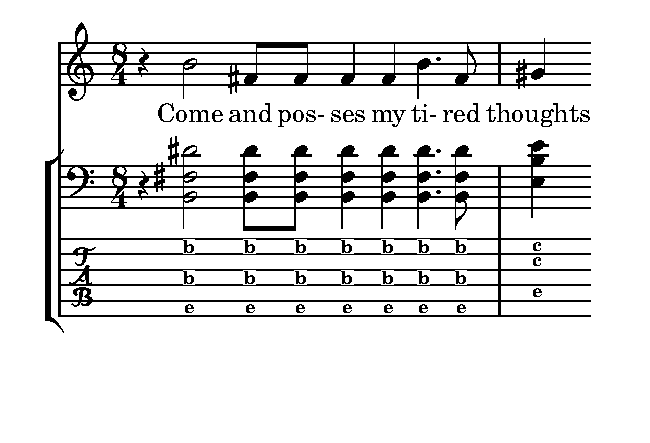
\includegraphics{examples/come.pdf}
\label{dowland-come}
\caption{``Come heavy sleep'' from \textit{The First Booke of Songs or Ayres} (1597), mm. 9}
\end{figure}
In figure~\ref{dowland-come}, there are repeat instances of F$\sharp$ and D$\sharp$ in the
first measure of our example, which are represented in the tablature part by the character
\textit{b}.  English lute music was written in the French system of tablature, so the
frets are indicated with letters.  The tablature character \textit{a} being the open
string and the character \textit{b} is the first fret.  If we were trying to follow the
meantone fretting system I outlined earlier, these notes would be G$\flat$ and E$\flat$
and would sound quite strident against the B.  Recalling Dowland's own choice for the
first fret, as shown in table~\ref{table:comparison}, the quality of semitone is diatonic,
but is in sixth-comma and not quarter-comma.  A sixth-comma fret would certainly be more
palatable in this case and is perhaps why Dowland himself was advocating for a sixth-comma
diatonic semitone instead of a quarter-comma one.

Other examples from Dowland's ouvre highlight the central problem with employing meantone
fretting systems on lutes.  Because of how fretted instruments are tuned, there are cases
when both the diatonic and chromatic semitone are required at the same fret. For example,
in his song \textit{I saw my lady weepe}, there are both G minor chords and D major
chords, which require a B$\flat$ and the F$\sharp$.   However, if look at an excerpt from
the sone below, we can see that these notes are both placed on the same fret.
\begin{figure}[h]
\centering
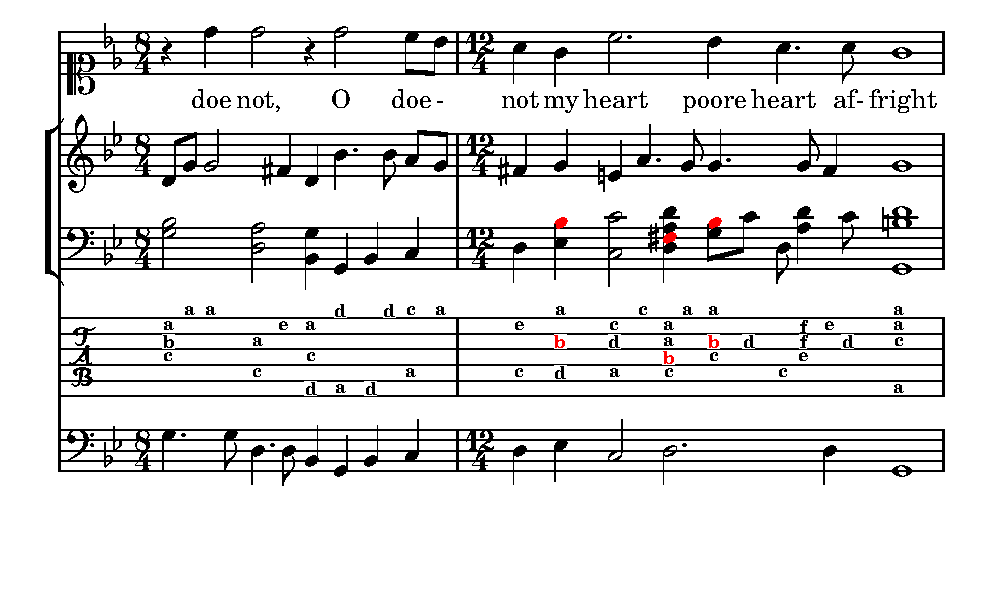
\includegraphics{examples/saw.pdf}
\label{dowland-saw}
\caption{``I saw my lady weepe'' from \textit{The Second Booke of Songs or Ayres} (16??), mm. 9}
\end{figure}
The notes and their corresponding tablature characters are highlighted in red.  Both notes
occur on the first fret, where there is the tablature character \textit{b}.  If we were to
use a meantone fretting system, the B$\flat$ would be true but the F$\sharp$ would be a
G$\flat$ instead, unless we were using a tastino to correct the problem. This kind of
issue results when frets determine the quality of the semitone regardless of what the
particular pitch might be.  Keyboard and other instruments are exempt from this kind of
issue because their semitones can be tuned independent of one another.  A keyboard or
organ can very easily have F$\sharp$ and B$\flat$ existing at the same time.

Referring back to Dowland's own fretting instructions from the first chapter, he did
recommend a sixth-comma diatonic semitone at the first fret which would ease the
problem of having the F$\sharp$ and B$\flat$ on the same fret.  Although the problem of having
a G$\flat$ instead of an F$\sharp$ would remain, the difference would not sound quite as
pronounced as a quarter-comma difference.  Since other composers and lute players
were subject to the same tuning constraints, it is understandable that some might have
opted for an equal semitone approach the would minimize the problems even further.
Yet, the ensemble problem still would have remained and applying an equal
semitone solution, or even a sixth-comma meantone solution, would mean that the lute
would be attempting to play in tune with an ensemble that was using a different
temperament.

The same issues that affect fretting systems for Renaissance lute also affect the theorbo
as well.  Although they are less common, there are tablature accompaniments for the
theorbo and just as we studied lute tablatures for clues regarding temperament choices,
we can also examine some of the theorbo accompaniment tablatures for the same information.
An example of an early seventeenth-century theorbo tablature accompaniment comes from
Girolamo Kapsberger, a theorbo player and composer who was active in Rome. In addition
to publishing several books of music for solo theorbo, he published
four books of villanelle written for for voices, bowed bass, guitar and theorbo.  The
vocal parts and bass part are written in staff notation, while the guitar and theorbo
parts are written in their own specialized notation.  In the case of the guitar,
alphabetic notation is used, where a series of different letters indicate which chord to play.
The theorbo part is in Italian-style tablature, where numbers are used in place of letters
to indicate fret placement and the order of strings is actually inverted from French-style
tablature so the top string of the theorbo is bottom line of the tablature staff.  For
sake of consistency, I have transcribed Kapsberger's tablature part into French tablature
so we can make comparisons between the examples with lute and theorbo.

The song ``All' ombra'', from his first book of villanelle, contains a cadence in A major
towards the end of the piece.  The G$\sharp$ and C that are used  are highlighted in red.
\begin{figure}[h]
\centering
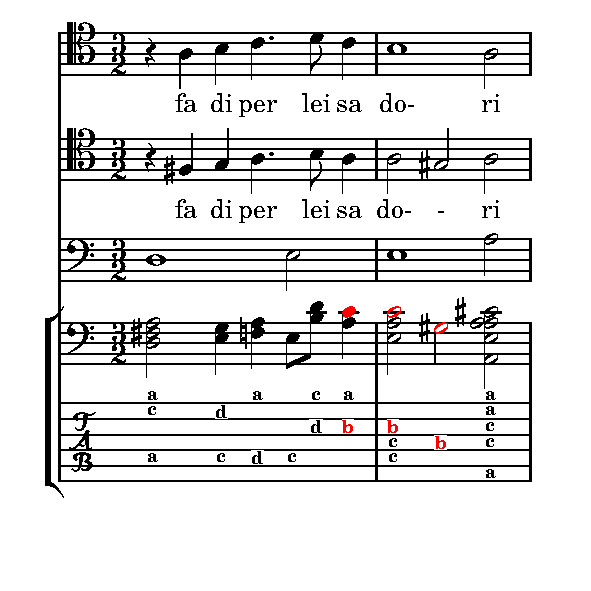
\includegraphics{examples/kaps_ombria.pdf}
\label{kaps-ombria}
\caption{``All' ombra'' from \textit{Di Villanelle, bk. 1} (16??), mm. 21-22 }
\end{figure}
Similar to our previous example from Dowland, these two notes are found on the same
fret, indicated with the tablature character \text{b} highlighted in red.  If we were
employing a meantone fretting on our theorbo, the G$\sharp$ would instead be an A$\flat$.
In this example, the sound of the theorbo in such a temperament was either accepted
or the instrument used a different temperament, such as sixth-comma or another kind of
temperament that used equal semitones, in order to make different between the G$\sharp$
a bit more palatable.

If Kapsberger's theorbo was definitely in quarter-comma meantone, as tastino would have
been the only solution to avoid the A$\flat$ issue on his first fret.  An alternative
solution that I proposed earlier would be to change the left-hand fingering of the
E major chord so that the G$\sharp$ on the fourth fret is used resulting in a chromatic
semitone and not a diatonic one.  However, Kapsberger's tablature clearly indicates
that the G$\sharp$ on the first fret is to be used.

These examples represent only a fraction of the type of problems that lute players
faced when tuning to meantone temperaments.  The problems of chromatic versus diatonic
frets were pervasive in the literature so that it would have been impossible to simply
ignore them.  When faced with the problem in a performance context, the player must
turn to any possible solution that could make it possible for a lute to play in an
ensemble tuned to a meantone temperament.  In the concluding chapter of this study,
I will examine these solutions and how they might be used in the context of various kinds
of ensembles in which the lute and theorbo played a part during the late sixteenth
and early seventeenth centuries.